\documentclass{article}

\usepackage[a4paper, left=1.5cm, right=1.5cm, top=2cm, bottom=2cm]{geometry}

\usepackage{../../../../components/components}
\usepackage{hyperref}
\usepackage{fancyhdr}


% Configuration des en-têtes et pieds de page
\pagestyle{fancy}
\fancyhf{} % reset tout

\fancyhead[L]{DL2 Math-Info ASF4}
\fancyhead[C]{Algèbre}
\fancyhead[R]{2025-2026}

\fancyfoot[L]{Ewen Rodrigues de Oliveira}
\fancyfoot[R]{\thepage}

\begin{document}

\docTitle{Chapitre 8 : Isométries et orientation des espaces euclidiens en dimensions 2 et 3}

\section{Espaces euclidiens orientés}
\subsection{Orientation d'un espace vectoriel}
\definition{
    Considérons la relation d'équivalence sur les bases \textit{ordonnées} d'un espace vectoriel $E$ suivante : $\mathcal{B} = (e_1, \ldots, e_n) \sim (e_1', \ldots, e_n') = \mathcal{B}'$ si et seulement si $det P_{\mathcal{B} \to \mathcal{B}'} > 0$.\\
    Une orientation d'un espace vectoriel $E$ est un choix de l'une des classes d'équivalence pour cette relation.
}
\remark{Donc choisir une orientation, c'est prendre une base orthonormée qu'on décrète \textbf{directe} et les autres bases de la même classe d'équivalence sont aussi directes. Les bases de l'autre classe d'équivalence sont dites \textbf{indirectes}.}
\example{
    $E = \mathbb{R}^2$ muni de $(\vec{i}, \vec{j})$ la base canonique.\\ L'orientation "classique" de $\mathbb{R}^2$ est la classe d'équivalence de $(\vec{i}, \vec{j})$ pour $\sim$.
    
    \begin{center}
        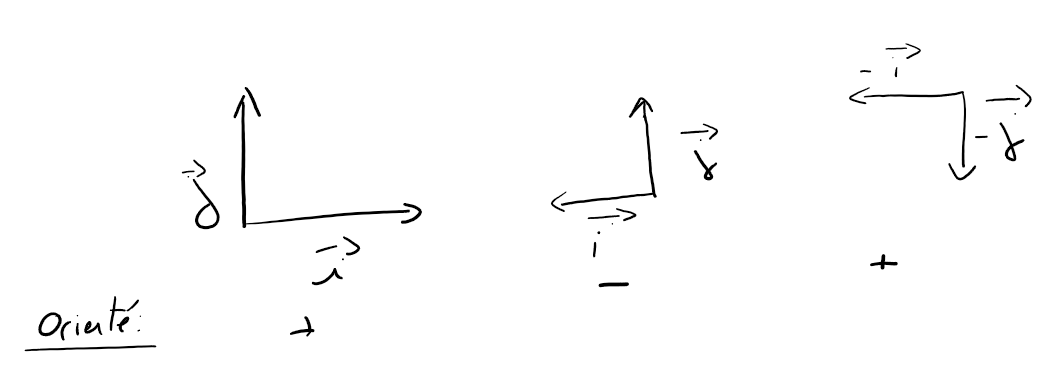
\includegraphics[width=0.5\textwidth]{./images/eg1.png}
        \captionof{figure}{Schéma de différentes orientations de $\mathbb{R}^2$}
    \end{center}
    L'orientation "classique" de $\mathbb{R}^3$ correspond à la "règle de la main droite". Une méthode plus sûre est de calculer le déterminant de la matrice de passage entre la base canonique et la base donnée.
}
\remark{De manière usuelle, on choisit toujours la base canonique de $\mathbb{R}^n$ pour définir l'orientation "classique" de $\mathbb{R}^n$.}

%\example{
%    $E = \mathbb{R}^3$ muni de $(\vec{i}, \vec{j}, \vec{k})$ la base canonique.\\ L'orientation "classique" de $\mathbb{R}^3$ correspond à la "règle de la main droite".
%    \begin{center}
%        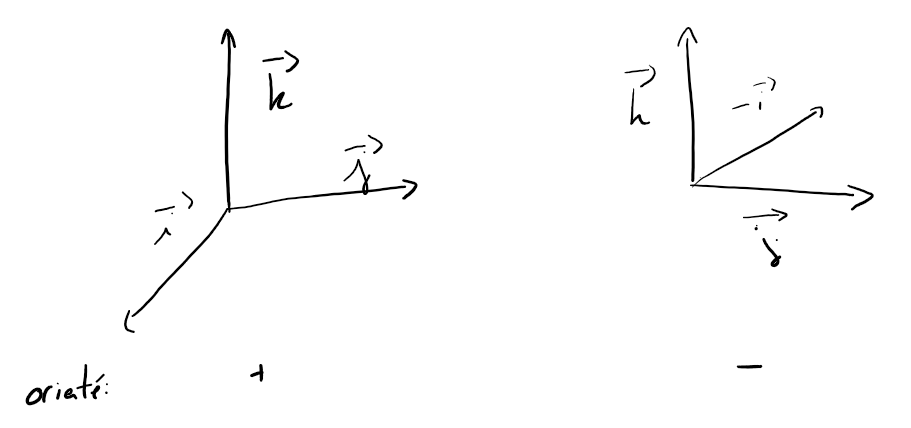
\includegraphics[width=0.5\textwidth]{./images/eg2.png}
%        \captionof{figure}{Schéma de différentes orientations de $\mathbb{R}^3$}
%    \end{center}
%}

\subsection{Espaces euclidiens et produits mixtes}
\subsubsection{Définition du produit mixte}
\vocabulary{Un \textbf{espace euclidien orienté} est un espace euclidien muni d'une orientation.}

\definition{
    Soient $x_1, \ldots x_n$ des vecteurs d'un espace euclidien orienté. On appelle \textbf{produit mixte} ou \textbf{déterminant} la quantité :
    \[
        Det(x_1, \ldots, x_n) = [x_1, \ldots, x_n] = det_{\mathcal{B}}(x_1, \ldots, x_n) \; \text{ où } \mathcal{B} \text{ est une base orthonormée directe quelconque de } E
    \]
}
\remark{On met bien $Det$ en majuscules pour le différencier du déterminant de matrices / de familles de vecteurs usuel.}

\subsubsection{Cas particulier de la dimension 2}

\example{
    Soit $E$ un espace euclidien orienté de dimension 2. Soient $x,y \in E$.\\
    Alors $[x,y] = \begin{vmatrix}
        x_1 & y_1 \\
        x_2 & y_2
    \end{vmatrix}$, où $(e_1, e_2)$ est une base orthonormée directe de $E$.
}

\theorem{Proposition}{Caractérisation du produit mixte en dimension 2}{false}{
    Soient $u,v \in E$.\\ Alors on a que $[u,v] = \langle u^\perp, v \rangle$.
}
\noindent{\textbf{Preuve :}\\
Soit $(e_1, e_2)$ une base orthonormée directe de $E$.\\
Posons $u = (x,y)$ et $v = (x',y')$ dans cette base.\\
Alors $u^\perp = (-y,x)$, et $\langle u^\perp, v \rangle = -yx' + xy' = [u,v]$. $\Box$
}

\remark{Le produit mixte représente l'aire du parallélogramme formé par les vecteurs $x$ et $y$, avec un signe qui dépend de l'orientation (sens trigonométrique ou sens horaire).}

\example{
    \begin{center}
        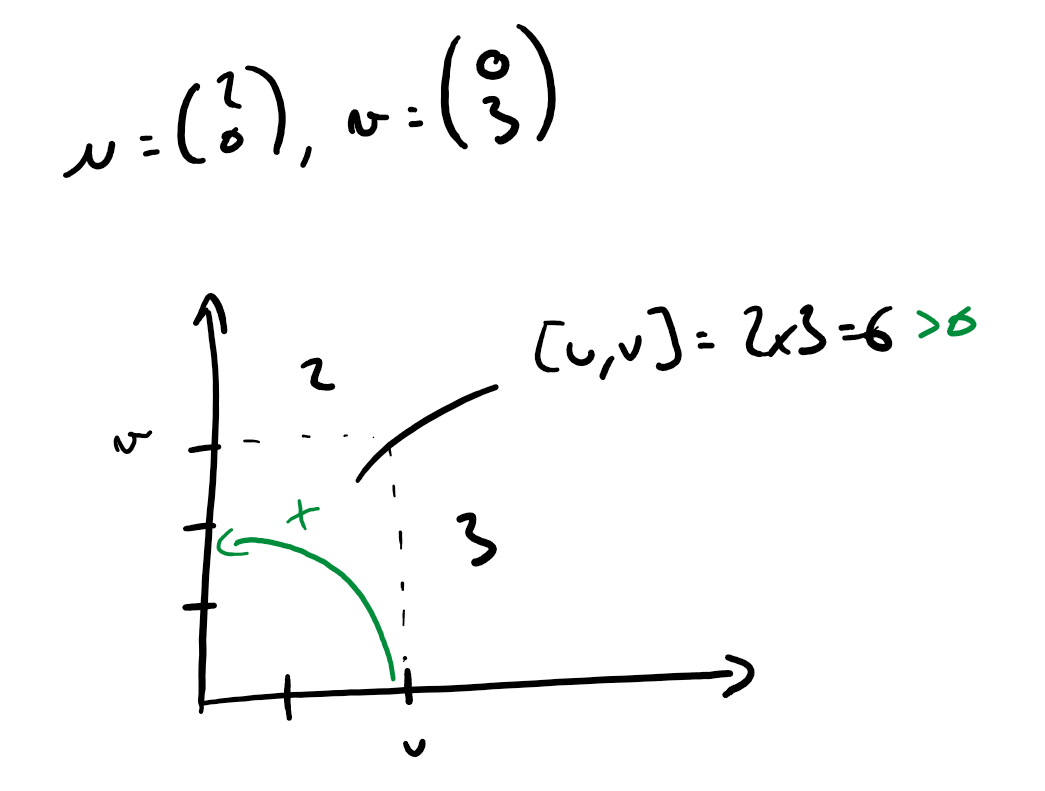
\includegraphics[width=0.25\textwidth]{./images/eg3.png}
        \captionof{figure}{Schéma du produit mixte (aire du rectangle) en dimension 2}
    \end{center}
}

\subsubsection{Cas particulier de la dimension 3 : le produit vectoriel}
Soit $E$ un espace euclidien orienté tel que $dim(E) = 3$.

\reminder{
    Théorème de représentation de Riesz: pour toute forme linéaire $f$ sur $E$, il existe un unique vecteur $v_f$ tel que pour tout $x \in E$, $f(x) = \langle v_f, x \rangle$.
}

\noindent Soient $x,y \in E$, alors : $z \mapsto [x,y,z]$ est une application linéaire.
On appliquant le théorème de représentation de Riesz, il existe un unique vecteur noté $x \wedge y$ tel que $\forall z \in E, [x,y,z] = \langle x \wedge y, z \rangle$. 

\definition{
    Soit $E$ un espace euclidien orienté de dimension 3. Soient $x,y \in E$.\\
    On appelle \textbf{produit vectoriel} de $x$ et $y$ le vecteur $x \wedge y$ défini par : $\forall z \in E, [x,y,z] = \langle x \wedge y, z \rangle$.
}
\attention{Le produit vectoriel n'est pas égal au produit mixte, mais il est défini à partir du produit mixte.}
\attention{Le produit vectoriel $\wedge$ n'est pas associatif. En revanche, si $a,b,c \in E$, on peut définir $a \wedge (b \wedge c) = \langle a, c \rangle b - \langle a, b \rangle c$.}

\theorem{Propriétés}{}{false}{
    \begin{enumerate}
        \item \function{*}{E \times E \to E}{(x,y) \mapsto x \wedge y} est une application bilinéaire antisymétrique.
        \item $\forall x,y,z \in E \; \langle x \wedge y, z \rangle = \langle z \wedge x, y \rangle = \langle y \wedge z, x \rangle$.
        \item $\langle x \wedge y, x \rangle = \langle x \wedge y, y \rangle = 0$.
        \item Si $\exists \lambda \in \mathbb{R}$ tel que $x = \lambda y$, alors $x \wedge y = 0$.
    \end{enumerate}
}


\training{Montrer que $\forall x,y,z \in E$, on a l'identité de Jacobi : $x \wedge (y \wedge z) + y \wedge (z \wedge x) + z \wedge (x \wedge y) = 0$.}
\noindent \carreaux{7}

\theorem{Proposition}{Calcul dans une B.O.N. directe}{false}{
    Soit $\mathcal{B} = (e_1, e_2, e_3)$ une base orthonormée directe de $E$.\\
    Alors pour tous $x,y \in E$, on a : $x \wedge y = (x_2y_3 - x_3y_2)e_1 + (x_3y_1 - x_1y_3)e_2 + (x_1y_2 - x_2y_1)e_3$.
}
\noindent{\textbf{Preuve:}\\
On pose $x = \sum_{i=1}^3 x_i e_i$ et $y = \sum_{i=1}^3 y_i e_i$.\\
$x \wedge y = \langle x \wedge y, e_1 \rangle e_1 + \langle x \wedge y, e_2 \rangle e_2 + \langle x \wedge y, e_3 \rangle e_3$\\

Or $\langle x \wedge y, e_1 \rangle = \begin{vmatrix}
x_1 & y_1 & 1 \\
x_2 & y_2 & 0 \\
x_3 & y_3 & 0
\end{vmatrix} = (x_2y_3 - x_3y_2)$, $\langle x \wedge y, e_2 \rangle = \begin{vmatrix}
x_1 & y_1 & 0 \\    
x_2 & y_2 & 1 \\
x_3 & y_3 & 0
\end{vmatrix} = (x_3y_1 - x_1y
_3)$ et $\langle x \wedge y, e_3 \rangle = \begin{vmatrix}
x_1 & y_1 & 0 \\
x_2 & y_2 & 0 \\
x_3 & y_3 & 1
\end{vmatrix} = (x_1y_2 - x_2y_1)$.\\
D'où $x \wedge y = \begin{vmatrix}
x_1 & y_1 & e_1 \\
x_2 & y_2 & e_2 \\
x_3 & y_3 & e_3
\end{vmatrix}$. $\Box$
}

\example{
    Soit $E = \mathbb{R}^3$ muni de la base canonique $(\vec{i}, \vec{j}, \vec{k})$.\\
    Soient $x = (1,2,3)$ et $y = (4,5,6)$.\\
    Alors $x \wedge y = (2 \cdot 6 - 3 \cdot 5)\vec{i} + (3 \cdot 4 - 1 \cdot 6)\vec{j} + (1 \cdot 5 - 2 \cdot 4)\vec{k} = (-3,6,-3)$.\\
    On vérifie que $\langle x \wedge y, x \rangle = \langle x \wedge y, y \rangle = 0$ et que $[x,y,z] = \langle x \wedge y, z \rangle$ pour tout $z \in E$.
}

\example{
    On pose $u = (1,0,1)$ et $v = (0,2,0)$.\\
    Notons $u \wedge v = (x,y,z)$.\\
    On a que :
    $\begin{vmatrix}
        1 & 0 & x \\
        0 & 2 & y \\
        1 & 0 & z
    \end{vmatrix} = -2x+2z$
    Donc $-2x+2z = 0$, d'où $u \wedge v = (2,0,2)$. (à une constante près).
}

\section{Étude du groupe des isométries en dimension 2 et 3}
\subsection{Groupe orthogonal d'un espace euclidien orienté}

On se place dans un espace euclidien $E$ muni du produit scalaire $\langle \cdot, \cdot \rangle$.\\
On étudie $O(E)$, spécialement pour les isométries de dimension 2 et 3.

\remark{$det$ est un morphisme de groupes, donc si $u \in O(E)$, $det(uu^*) = 1 = det(u)det(u^*) = det(u)^2$. Donc $det(u) \in \{-1, 1\}$. En particulier, $ker(det)$ est un sous-groupe de $O(E)$.}

\definition{
    On note et on appelle $SO(E) = O_{+}(E) = ker(det)$ le \textbf{groupe spécial orthogonal} de $E$. Ces éléments sont les isométries de $E$ de déterminant 1, qu'on appelle aussi les \textbf{isométries directes} de $E$.\\\\
    \textit{De manière analogue, on note $O_{-}(E) = O(E) \setminus O_{+}(E)$ les isométries de $E$ de déterminant -1, qu'on appelle aussi les \textbf{isométries indirectes} de $E$.}
}
\attention{$O_{-}(E)$ n'est pas un sous-groupe, car le produit de deux isométries indirectes est une isométrie directe.}

\theorem{Proposition}{Propriétés spectrales}{false}{
    Si $\lambda$ est une valeur propre (réelle ou complexe) de $u \in O(E)$, alors $|\lambda| = 1$. En particulier, les seules valeurs propres réelles possibles sont $1$ et $-1$.
}

\noindent\textbf{Preuve :}\\ Soit $x$ un vecteur propre associé à $\lambda$. On a $\langle u(x), u(x) \rangle = \langle \lambda x, \lambda x \rangle = \lambda \bar{\lambda} \langle x, x \rangle = |\lambda|^2 \|x\|^2$. Comme $u$ est une isométrie, $\|u(x)\| = \|x\|$, d'où $|\lambda|^2 = 1$. $\Box$

\subsection{Classification des isométries en dimension 2}
\subsubsection{Isométries directes}
On étudie ici le groupe $SO(\mathbb{R}^2)$, c'est à dire le groupe des isométries directes de $\mathbb{R}^2$ \textit{(parfois écrit $SO_2(\mathbb{R})$)}.

\theorem{Théorie des rotations}{}{false}{
    Soit $u \in SO(\mathbb{R}^2)$. Alors il existe un unique $\theta \in ]-\pi, \pi]$ tel que la matrice de $u$ dans toute base orthonormée directe est de la forme :
    \[ R_\theta = \begin{pmatrix}
        \cos \theta & -\sin \theta \\
        \sin \theta & \cos \theta
    \end{pmatrix} \].
}

\noindent\textbf{Preuve :}\
Soit $u\in SO_2(\mathbb{R})$ et $(e_1, e_2)$ une base orthonormée directe. Posons $u(e_1) = \begin{pmatrix} a \\ b \end{pmatrix}$.\\
Comme $\|u(e_1)\| = 1$, on a $a^2 + b^2 = 1$.\\
Il existe donc un unique $\theta \in ]-\pi, \pi]$ tel que $a = \cos \theta$ et $b = \sin \theta$.\\\\
Or $u \in O(E)$, donc $u(e_2)$ doit être orthogonal à $u(e_1)$, donc $u(e_2) = \begin{pmatrix} -\sin \theta \\ \cos \theta \end{pmatrix}$ ou $u(e_2) = \begin{pmatrix} \sin \theta \\ -\cos \theta \end{pmatrix}$.\\
Or $\det(u) = 1$, ce qui impose la première solution. Donc la matrice de $u$ est bien $R_\theta$.

\vocabulary{On appelle $\theta$ l'angle de rotation de $u$. On appelle les éléments de $SO_2(\mathbb{R})$ les \textbf{rotations} du plan.}

\theorem{Proposition}{}{false}{
    $SO_2(\mathbb{R})$ est un groupe abélien isomorphe à $(\mathbb{R}/2\pi\mathbb{Z}, +)$.
}
\noindent\textbf{Preuve :}\
L'application $\varphi: \theta \mapsto R_\theta$ est un morphisme de groupes surjectif de noyau $2\pi\mathbb{Z}$. Par le premier théorème d'isomorphisme, $SO_2(\mathbb{R}) \simeq \mathbb{R}/2\pi\mathbb{Z}$. $\Box$

\subsubsection{Isométries indirectes}
\theorem{Classification des isométries indirectes}{}{false}{
Soit E un plan euclidien orienté. Toute isométrie indirecte $s \in O_{-}(E)$ est une réflexion (symétrie orthogonale par rapport à une droite).
}

\noindent\textbf{Preuve :}\
Soit $s\in O_{-}(E)$. Son polynôme caractéristique est $\chi_s(X)=X^2-Tr(s)X-1$.\\
Le discriminant $\Delta=Tr(s)^2+4$ est strictement positif, donc $s$ possède deux valeurs propres réelles distinctes.\\
Le produit des valeurs propres étant égal à $\det(s)=-1$, et les seules valeurs propres possibles pour une isométrie étant 1 ou -1, on en déduit que $Sp(s)=\{1,-1\}$.\\\\
$s$ est donc une symétrie par rapport à la droite $D = \ker(s - id_E)$ parallèlement à la droite $D'=\ker(s + id_E)$.\\
Puisque $s$ est une isométrie, les sous-espaces propres sont orthogonaux : $D'=D^\perp$.\\
$s$ est donc la réflexion d'axe $D$. $\Box$

\theorem{Proposition}{Forme matricielle}{false}{
Dans une base orthonormée directe quelconque, la matrice d'une réflexion est de la forme :
\[ S_\theta = \begin{pmatrix}
\cos \theta & \sin \theta \\
\sin \theta & -\cos \theta
\end{pmatrix} \]
Elle est toujours de trace nulle, et de déterminant égal à -1.
}

\vocabulary{On appelle $\theta$ l'angle de la réflexion $s$ et l'axe de symétrie de $s$ est la droite $\Delta = \ker(s - id_E)$.}

\remark{Contrairement aux rotations, le produit de deux réflexions n'est pas une réflexion, mais une rotation. $O_{-}(E)$ n'est donc pas un groupe.}

\subsection{Classification des isométries en dimension 3}
\subsubsection{Isométries directes}
Commençons par $E = \mathbb{R}^3$ et déterminons $SO(3) = SO_3(\mathbb{R})$. Soit $u \in SO_3(\mathbb{R})$. Alors $Sp(u) \subset \{-1, 1\}$.\\


\definition{On dira que $(e_1, e_2)$ base de $n^\perp$ est directe si $(e_1, e_2, n)$ est une base directe de $E$ \textit{(on parle aussi d'orientation induite sur $n^\perp$)}.}
\remark{Si $u \in SO_3(\mathbb{R})$, alors $1 \in Sp(u)$ \textit{(c'est primordial pour démontrer le théorème qui suit)}.}

\theorem{Théorème}{}{false}{
    Dans un espace euclidien orienté $E$ de dimension 3, une isométrie directe non triviale (une rotation en dimension 3), est déterminée par la donnée de :
    \begin{itemize}
        \item un axe orienté, c'est à dire un choix de vecteur unitaire $d$ dirigeant la droite $D = ker(u - id_E)$
        \item un angle de rotation $\theta \in ]-\pi, \pi]$
    \end{itemize}
    L'orientation de l'axe détermine une orientation du plan $D^\perp$ et si $(e_1, e_2)$ est orthonormée directe dans $D^\perp$ alors la matrice de $u$ dans la base $(d,e_1,e_2)$ est de la forme $\begin{pmatrix}
        1 & 0 & 0 \\
        0 & \cos \theta & -\sin \theta \\
        0 & \sin \theta & \cos \theta
    \end{pmatrix}$.
}
\vocabulary{On appelle les éléments de $SO_3(\mathbb{R})$ les \textbf{rotations} de l'espace.}
\remark{Une conséquence importante de cela est que toute isométrie directe de $\mathbb{R}^3$ est une rotation autour d'un axe.}

\example{
    Soit $M \in \mathcal{SO}_3(\mathbb{R})$ la matrice d'une rotation telle que :
\[ M = \frac{1}{3}\begin{pmatrix}
    2 & -1 & 2 \\
    2 & 2 & -1 \\
    -1 & 2 & 2
\end{pmatrix} \]

    \textbf{1. Recherche de l'axe $\Delta$}
    $\ker(3(M - I_3)) = Vect((1,1,1))$. Posons $d = (1,1,1)$, alors $d$ est un vecteur directeur de l'axe de rotation $\Delta$. (la constante $3$ ne joue aucun rôle)\\

    \textbf{2. Détermination de la valeur absolue de $\theta$}
    On utilise la trace de la matrice $M$ qui est la même dans toutes les bases.\\
    $ \text{Tr}(M) = 1 + 2\cos\theta \implies \cos\theta = \frac{\text{Tr}(M) - 1}{2} = \frac{\frac{6}{3} - 1}{2} = \frac{1}{2}$.\\
    Donc $\theta \in \{-\frac{\pi}{3}, \frac{\pi}{3}\}$.\\

    \textbf{3. Détermination du signe de $\theta$ (Produit Mixte)}
    Pour trancher, on étudie le signe de $\sin\theta$. On choisit un vecteur $x$ non colinéaire à $d$ (souvent $e_1$) et on calcule le produit mixte :
    Prenons $x = e_1$, alors :
    \[ [{d}, {x}, u({x})] = \det({d}, {x}, M{x}) = \begin{vmatrix}
        1 & 1 & \frac{2}{3} \\
        1 & 0 & \frac{2}{3} \\
        1 & 0 & -\frac{1}{3}
    \end{vmatrix} = 1 \]

    \noindent Le signe du produit mixte est le même que celui de $\sin\theta$, donc $\sin\theta > 0$.\\
    Donc $\theta > 0$, il s'ensuit que $\theta = \frac{\pi}{3}$.\\
    Plus généralement, on a :
    \begin{itemize}
        \item Si $\det(d, x, M(x)) > 0 \implies \sin\theta > 0 \implies \theta = \frac{\pi}{3}$
        \item Si $\det(d, x, M(x)) < 0 \implies \sin\theta < 0 \implies \theta = -\frac{\pi}{3}$
    \end{itemize}
}

\subsubsection{Isométries indirectes}

\theorem{Lemme}{}{false}{
    Une isométrie indirecte est soit une réflexion, soit la composée d'une réflexion et d'une rotation. Dans ce cas on parle d'\textbf{anti-rotation}.
}
\noindent{\textbf{Preuve :}\\
Soit $u \in O_{-}(E)$. Par un raisonnement similaire au cas de $SO_3(\mathbb{R})$, on trouve que $-1 \in Sp(u)$. Raisonnons maintenant sur $dim(ker(u + id_E))$ :
\begin{itemize}
    \item Si $dim(ker(u + id_E)) = 3$, alors $u = -id_E$.
    \item Si $dim(ker(u + id_E)) = 2$ : impossible (car $u$ est une isométrie, donc les sous-espaces propres sont orthogonaux, et $ker(u + id_E) = ker(u - id_E)^\perp$).
\end{itemize}
Il reste à étudier le cas où $dim(ker(u + id_E)) = 1$. Soit $s$ la réflexion orthogonale par rapport à $ker(u + id_E)^\perp$.\\
Considérons l'isométrie directe $S$, alors $S \circ u = s$ est une rotation. Ainsi, $u$ est soit une réflexion (si $S = id_E$), soit la composée d'une réflexion et d'une rotation (si $S \neq id_E$). $\Box$
}

\theorem{Théorème}{}{false}{
    Soit $u \in O_{-}(E)$, alors :
    \begin{itemize}
        \item soit $u = -id_E$,
        \item Soit $dimKer(u+id_E) = 1$ et si $d$ est un vecteur unitaire engendrant cette droite (choix d'axe orienté), alors il existe un unique $\theta \in ]-\pi, \pi]$ tel que si $(e_1, e_2)$ est une base orthonormée directe de $d^\perp$ par d'orientation induite alors la matrice de $u$ dans la base $(d, e_1, e_2)$ est de la forme $\begin{pmatrix}
            -1 & 0 & 0 \\
            0 & \cos \theta & -\sin \theta \\
            0 & \sin \theta & \cos \theta
        \end{pmatrix}$.
    \end{itemize}
}
\remark{On a ces quelques cas particuliers :
    \begin{itemize}
    \item Si $\theta=0$, $u$ est une \textbf{réflexion} par rapport au plan $d^\perp$.
    \item Si $\theta=\pi$, $u=-id_E$ est la \textbf{symétrie centrale}.
    \end{itemize}
}
\theorem{Proposition}{Classification par la trace}{false}{
Soit $M \in O_3^-(\mathbb{R})$.
\begin{itemize}
    \item Si $Tr(M) = 1$, $M$ est une \textbf{réflexion} par rapport au plan $\ker(M-I_3)$.
    \item Si $Tr(M) = -3$, $M = -I_3$ est la \textbf{symétrie centrale}.
    \item Sinon, $M$ est une \textbf{anti-rotation} d'angle $\theta$ tel que $Tr(M) = -1 + 2\cos\theta$.
\end{itemize}
}

\noindent{\textbf{Démonstration pour la réflexion :}\\
Une réflexion $s$ a pour valeurs propres $(1, 1, -1)$. Sa trace est donc $1+1+(-1) = 1$. Réciproquement, si $u \in O_3^-$ et $Tr(u)=1$, alors $-1 + 2\cos\theta = 1 \implies \cos\theta = 1$, soit $\theta=0$. La matrice dans la base adaptée est donc $diag(-1, 1, 1)$, ce qui correspond bien à une réflexion par rapport au plan $Vect(e_1, e_2)$. $\Box$
}

\example{
    Soit $C \in O_3^-(\mathbb{R})$ la matrice suivante :
    \[ C = \frac{1}{9}\begin{pmatrix} 7 & 4 & 4 \\ -4 & 8 & -1 \\ 4 & 1 & -8 \end{pmatrix} \]

    \textbf{1. Nature de l'isométrie} \\
    $\det(C) = -1$ (isométrie indirecte) et $Tr(C) = \frac{1}{9}(7+8-8) = \frac{7}{9}$.\\
    Comme $Tr(C) \neq 1$, $C$ est une \textbf{anti-rotation}.

    \textbf{2. Recherche de l'axe $d$} \\
    On cherche $d$ tel que $Cu = -d$, soit $d \in \ker(C + I_3)$.
    \[ (C+I_3)X = 0 \iff \begin{pmatrix} 16 & 4 & 4 \\ -4 & 17 & -1 \\ 4 & 1 & 1 \end{pmatrix} \begin{pmatrix} x \\ y \\ z \end{pmatrix} = 0 \]
    Les lignes 1 et 3 donnent $4x + y + z = 0$. La ligne 2 donne $-4x + 17y - z = 0$.
    Par somme, $18y = 0 \implies y=0$, d'où $z = -4x$.
    On choisit l'axe orienté par $d = \begin{pmatrix} 1 \\ 0 \\ -4 \end{pmatrix}$.

    \textbf{3. Détermination de l'angle $\theta$} \\
    $Tr(C) = -1 + 2\cos\theta \implies \frac{7}{9} = -1 + 2\cos\theta \implies \cos\theta = \frac{8}{9}$.\\
    Ainsi $\theta = \pm \arccos(\frac{8}{9})$.

    \textbf{4. Signe de l'angle} \\
    On calcule le produit mixte $[d, e_2, C(e_2)]$ avec $e_2 = (0,1,0)^T$ :
    \[ \det(d, e_2, C e_2) = \begin{vmatrix} 1 & 0 & 4/9 \\ 0 & 1 & \frac{8}{9} \\ -4 & 0 & 1/9 \end{vmatrix} = \frac{1}{9} - (-4)(\frac{4}{9}) = \frac{17}{9} > 0 \]
    Le sinus est positif, donc $\theta = \arccos(\frac{8}{9})$.
}
\newpage
\tableofcontents

\end{document}